\newpage
\section{Test 3}
\label{Sec:test_3}

In the third test setting rover's parcour is divided into six time intervals with different values of torques applied to the wheels:

\begin{enumerate} 
  \item $0s < t_s < 20s$, $\tau = 0Nm$           
  \item $20s < t_s < 40s$, $\tau = 0.0007Nm$        
  \item $40s < t_s < 80s$, $\tau = 0Nm$         
  \item $80s < t_s < 105s$, $\tau = -0.0007Nm$
  \item $105s < t_s < 150s$, $\tau = 0Nm$         
  \item $150s < t_s < 200s$, $\tau = -0.0005Nm$ 
\end{enumerate}

\noindent Other external forces acting on the rover are the gravity and ground reactions. Initial position of the center of mass of the robot
has been set to (x, y, z) = (5, 8, 0.57) [m]. In the $5^{th}$ phase rover effectively stops its motion until negative torques are applied.
Friction coefficient has been set to 0.7. Restitution coefficients (tangential and normal) have been set to zero. 

\begin{figure}[H]
  \centering
    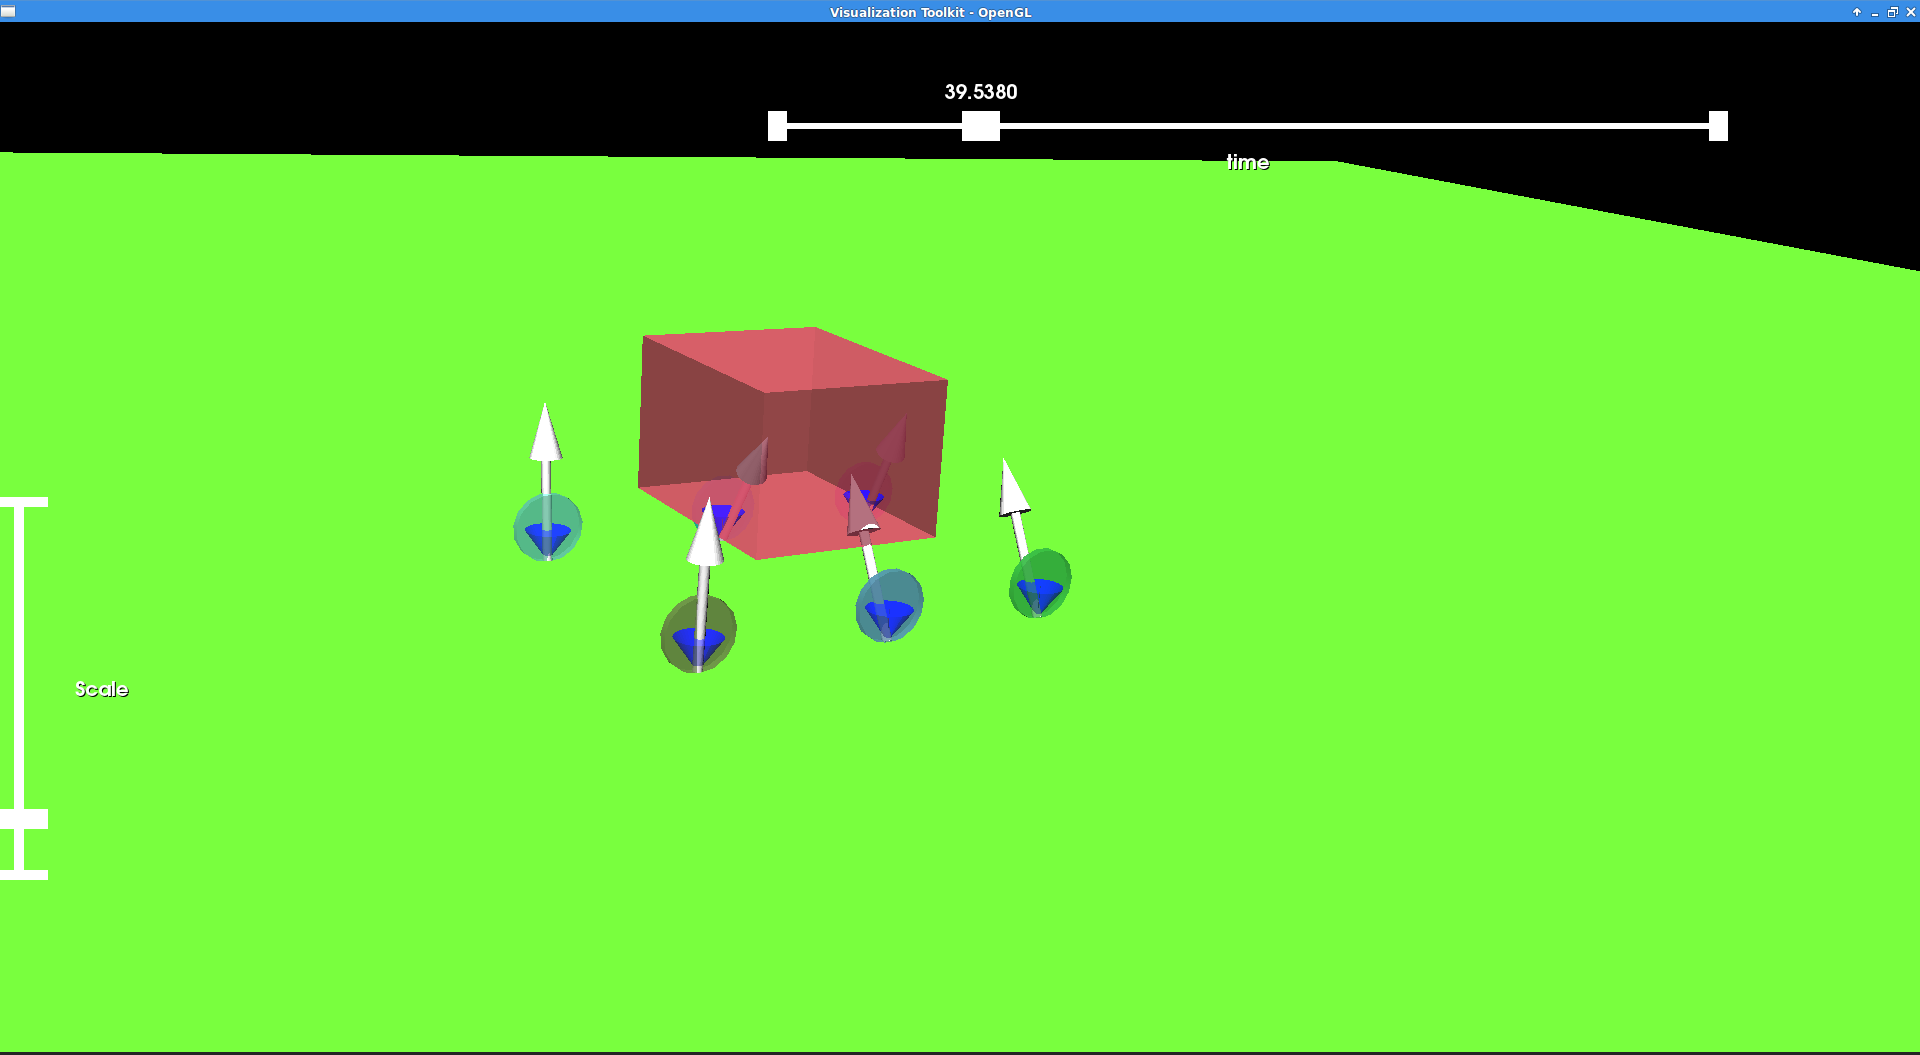
\includegraphics[width=0.8\textwidth]{run_3}
  \caption{Third test scenario (arrows depict contact forces)}
\end{figure}

\noindent In this case, following quantities have been plotted:

\begin{figure}[H]
  \centering
    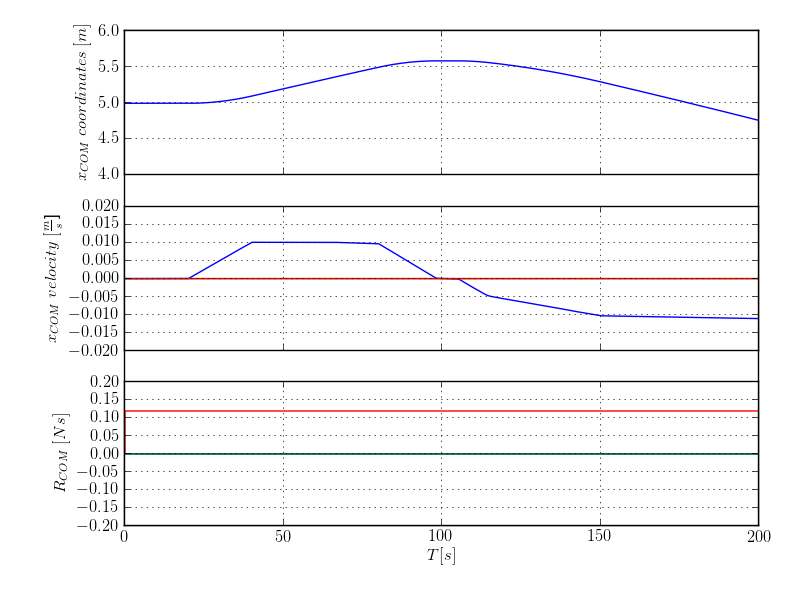
\includegraphics[width=0.8\textwidth]{xvpCOM3}
  \caption{Position, velocity and reaction forces of the center of mass}
\end{figure}

\noindent \textbf{\textit{\Large{Comments}}}\\[1mm]
\noindent Rover's motion has been divided into six phases. Figure 15 depicts those phases in terms of the center of mass velocity. Phases 2 and 3 represent forward motion with 
a constant velocity in the third phase. In the fourth phase rover moves in the opposite direction with a linear velocity to effectively stop in the fifth phase of motion.\\

\noindent Following additional quantities have also been plotted:

\begin{figure}[H]
  \centering
    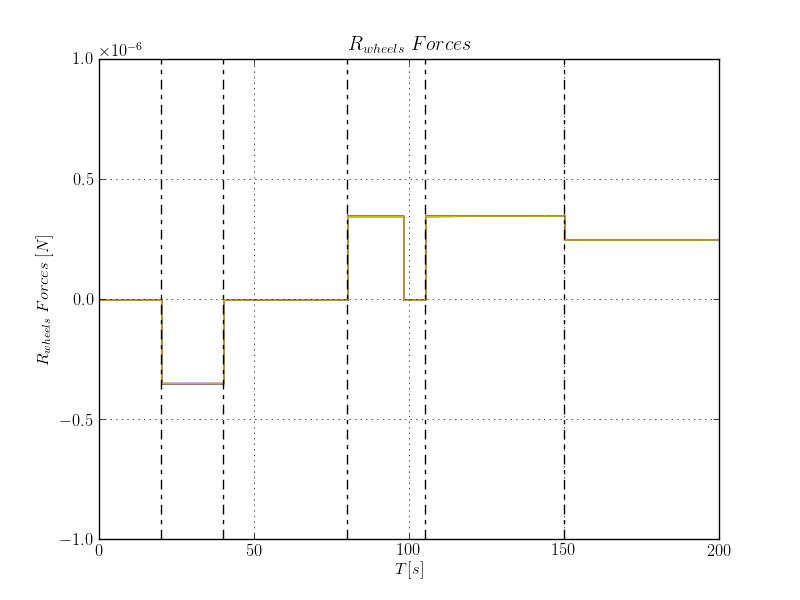
\includegraphics[width=0.8\textwidth]{pWHEELS3}
  \caption{$R_{wheels}$ - reaction forces (impulsions) of wheels in lagrangian coordinates}
\end{figure}

\begin{figure}[H]
  \centering
    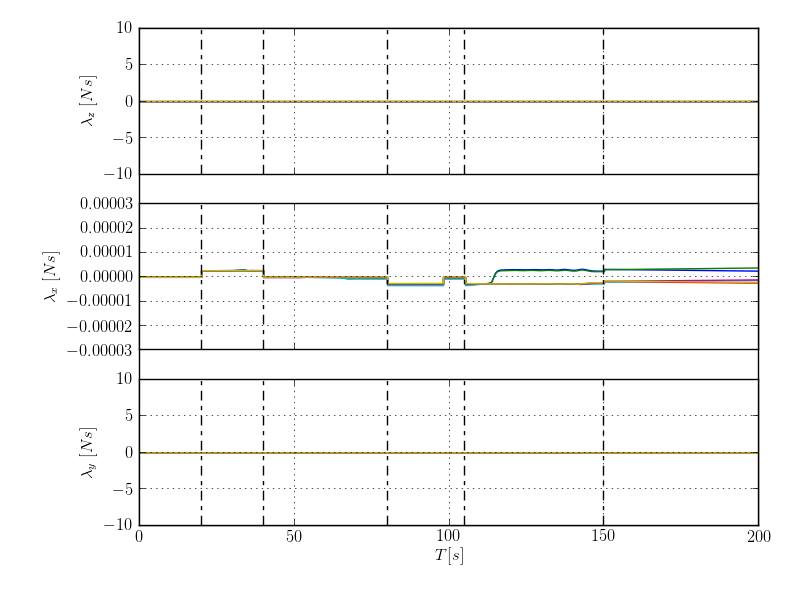
\includegraphics[width=0.8\textwidth]{lambdaNTS3}
  \caption{$\lambda_{N}$, $\lambda_{T_{x}}$, $\lambda_{T_{y}}$ - normal and tangential components of the contact force (impulsion) for each wheel}
\end{figure}

\noindent \textbf{\textit{\Large{Comments}}}\\[1mm]
\noindent In the figure 16 one can see the step pattern of the reaction torques resulting from the fact that the rover is moving along the x axis. Jumps in value represent changes in the friction force along x axis as torques 
are applied to the wheels. In the figure 17 all components of the local contact forces are displayed. Step pattern along x axis can be observed.
